%%%%%%%%%%%%%%%%%%%%%%%%%%%%%%%%%%%%%%%%%
% Friggeri Resume/CV
% XeLaTeX Template
% Version 1.2 (3/5/15)
%
% This template has been downloaded from:
% http://www.LaTeXTemplates.com
%
% Original author:
% Adrien Friggeri (adrien@friggeri.net)
% https://github.com/afriggeri/CV
%
% License:
% CC BY-NC-SA 3.0 (http://creativecommons.org/licenses/by-nc-sa/3.0/)
%
% Important notes:
% This template needs to be compiled with XeLaTeX and the bibliography, if used,
% needs to be compiled with biber rather than bibtex.
%
%%%%%%%%%%%%%%%%%%%%%%%%%%%%%%%%%%%%%%%%%

\documentclass[]{friggeri-cv} % Add 'print' as an option into the square bracket to remove colors from this template for printing

\addbibresource{mathdugrecv.bib} % Specify the bibliography file to include publications

\begin{document}

\header{Mathieu}{Dugré}{Software Developer} % Your name and current job title/field

%----------------------------------------------------------------------------------------
%	SIDEBAR SECTION
%----------------------------------------------------------------------------------------

\begin{aside} % In the aside, each new line forces a line break
	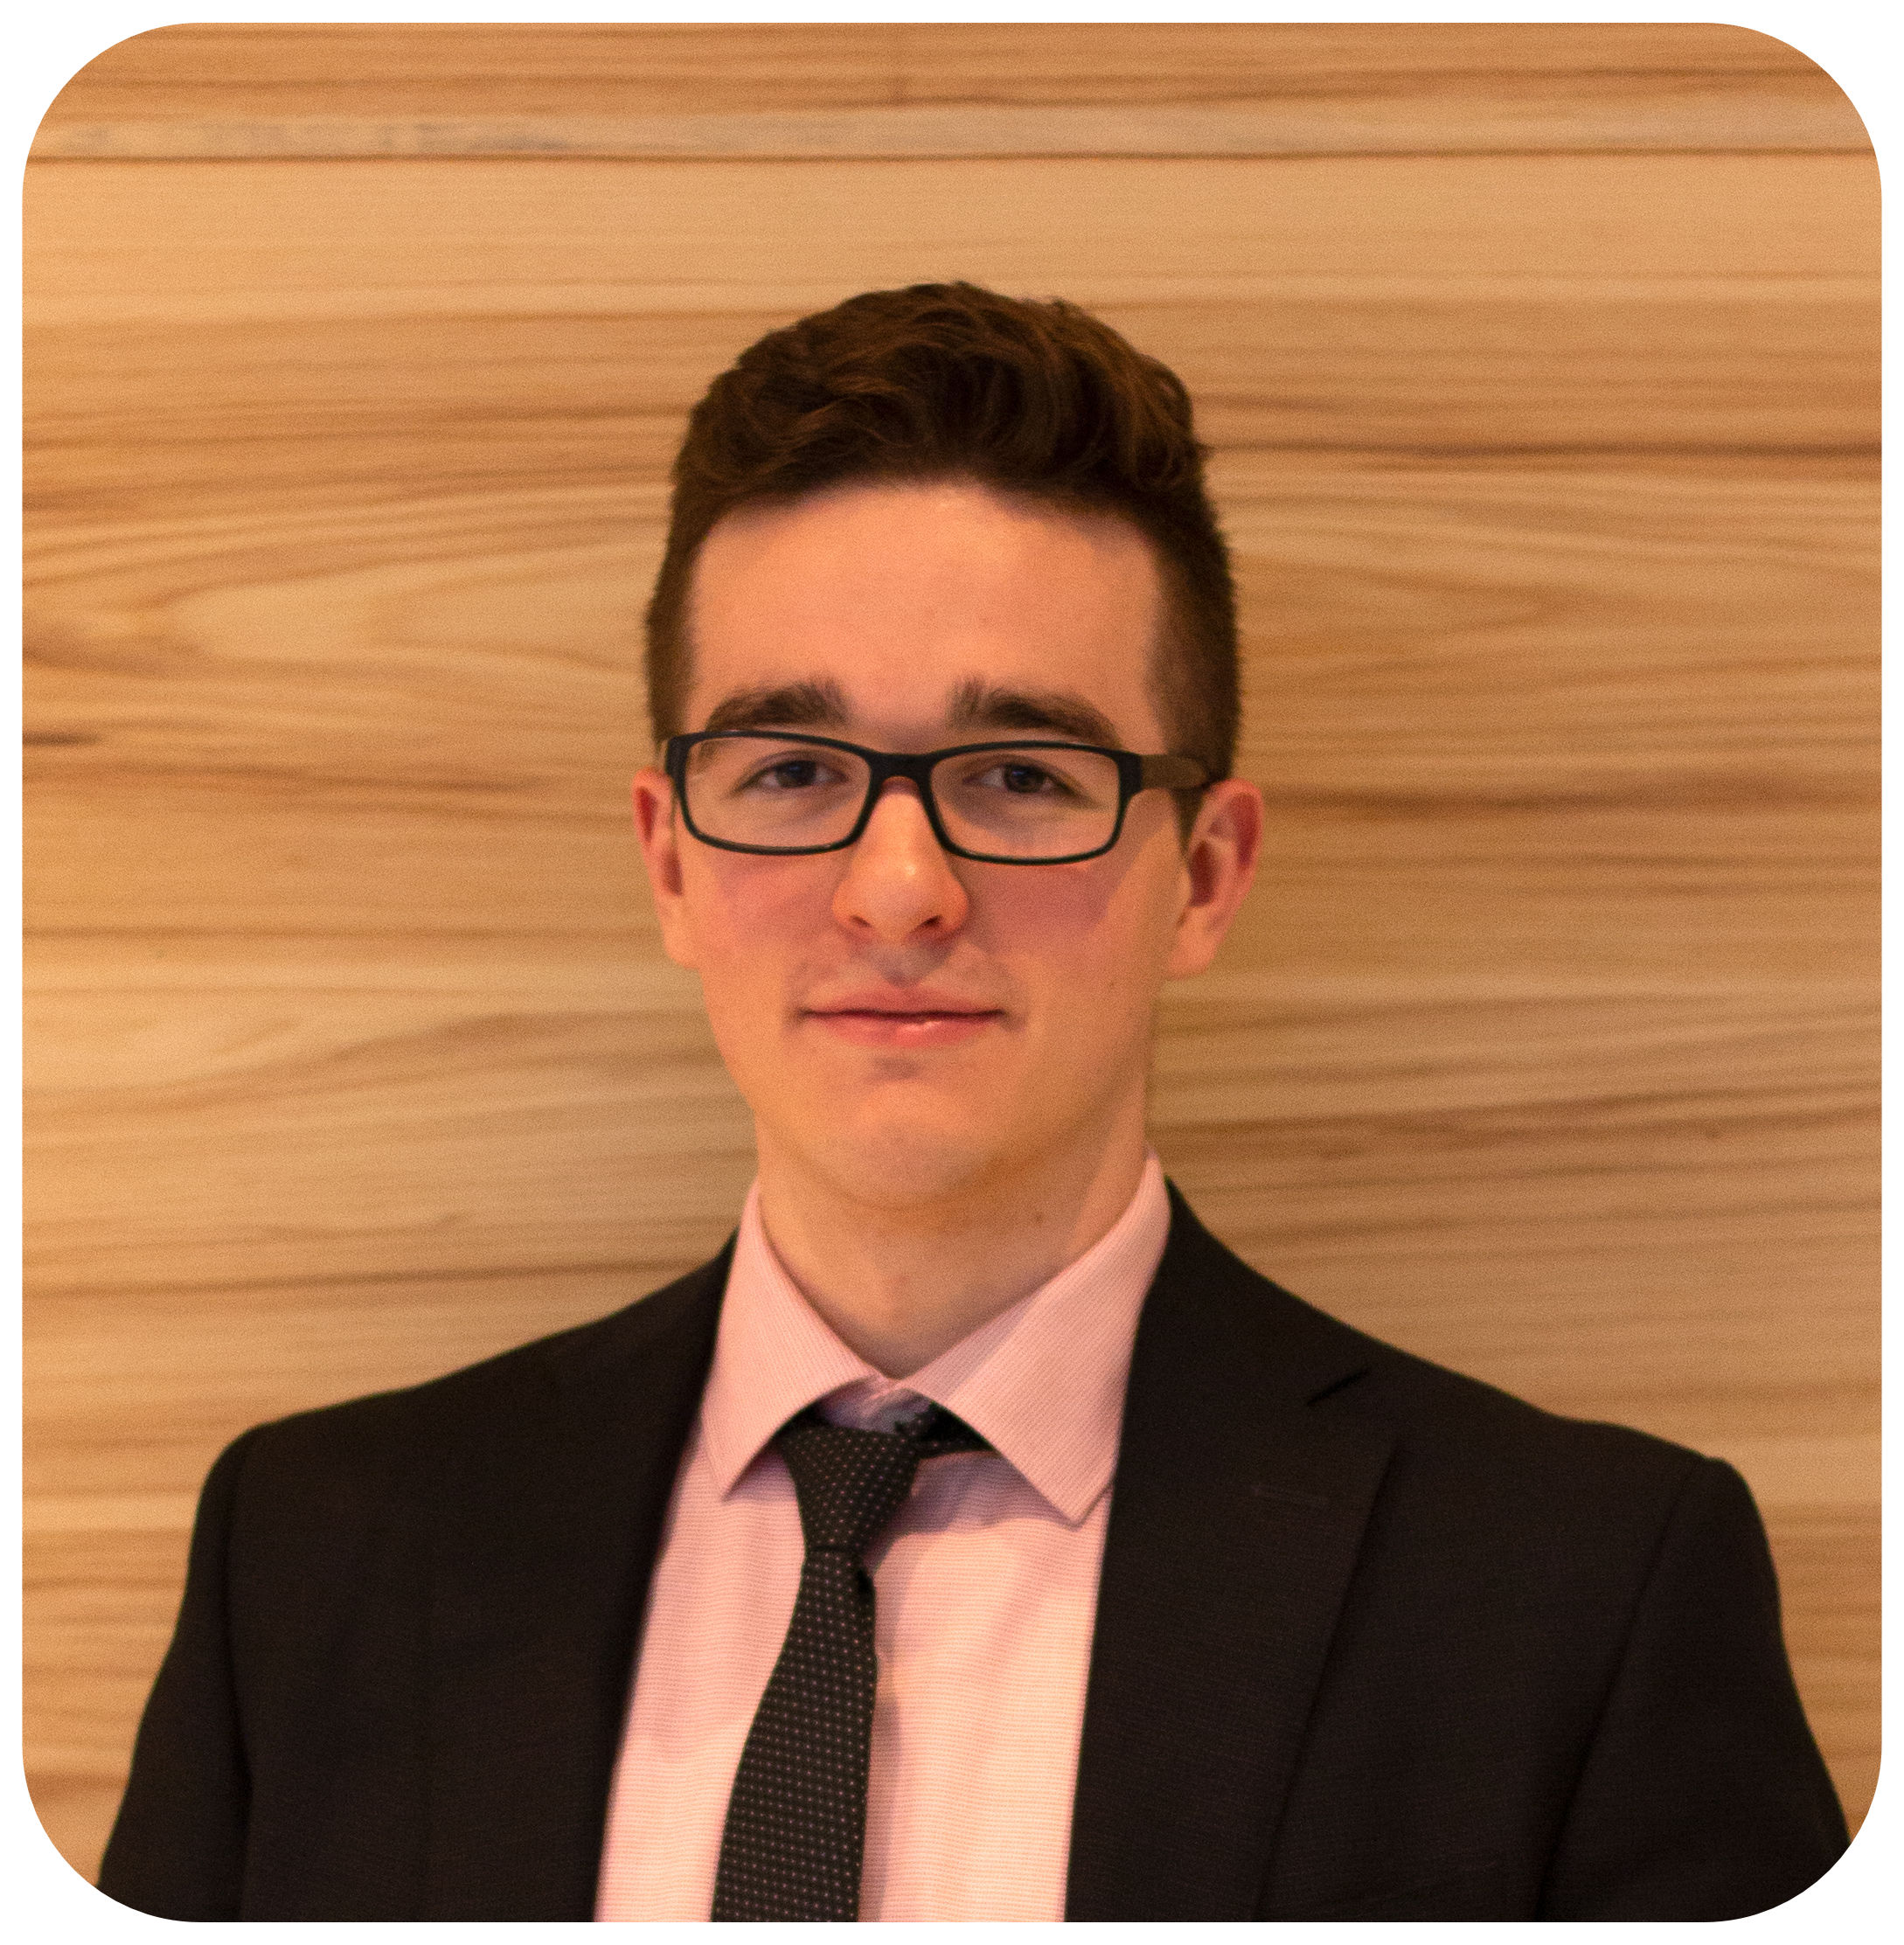
\includegraphics[width=\textwidth]{./photo-rounded_rectangle.jpg}
	\section{Contact}
	6590A rue Louis-Dupire
	Montreal, Quebec
	H1M 1A6, Canada
	~
	\href{mailto:mathdugre@pm.me}{mathdugre@pm.me~{\color{red} \faEnvelope}}
	\href{https://mathdugre.me}{mathdugre.me~{\color{lightblue} \faGlobe}}
	\href{https://github.com/mathdugre}{mathdugre~{\color{purple} \faGithub}}
	\href{https://twitter.com/mathdugre}{{\color{blue} \faTwitter}} \href{https://www.linkedin.com/in/mathdugre}{{\color{green} \faLinkedin}} \href{https://scholar.google.com/citations?user=QVPqTAsAAAAJ&hl=en}{{\color{googred} \aiGoogleScholar}}
	\section{Languages}
	French native
	English bilingual
	\section{Programming}
	Python, Docker, Linux {\color{red} $\varheartsuit$}
	Dask, Bash, \LaTeX
	\section{Soft skills}
	leadership, management, communication, problem~solving
	\section{Research interests}
	Performance, HPC, Data~locality, Distributed~systems
	\section{Personal interests}
	Reading, Running, Baking, Cooking, Language learning
\end{aside}

%----------------------------------------------------------------------------------------
%	EDUCATION SECTION
%----------------------------------------------------------------------------------------

\section{Education}
\begin{entrylist}
																											
	%------------------------------------------------
																											
	\entry
	{2020--now}
	{M.Comp.Sci.}
	{Concordia University, Montreal, QC}
	{Thesis work supervised by Dr. Tristan Glatard. 
	Studying strategies to improve data locality in HPC environment.}
																											
	%------------------------------------------------
																											
	\entry
	{2017-- 2020}
	{B.Comp.Sci. {\normalfont Honours Computer Aplications}}
	{Concordia University, Montreal, QC}
	{Major in Mathematics and Statistics.\\
		Honours work supervised by Dr. Tristan Glatard on a project to minimize 
		the data transfer of container applications in High Performance 
	Computing environment.}
																											
	%------------------------------------------------
																											
\end{entrylist}

%----------------------------------------------------------------------------------------
%	WORK EXPERIENCE SECTION
%----------------------------------------------------------------------------------------

\section{Experience}

\subsection{Academic experience}
\begin{entrylist}
																											
	%------------------------------------------------
																											
	\entry
	{2019 -- now}
	{Concordia University}
	{Montreal, QC}
	{\job{Research Assistant with Dr. Tristan Glatard} \\
		• Help to administrate the compute cluster of our lab.\\
		• Built a tool helping PERFORM Center researchers to share restricted 
		data on CONP portal.\\
		• Published and presented a paper at WORKS'19 on the performance of two 
		Big Data engines Dask and Apache Spark.
	}
																											
	%------------------------------------------------
																											
\end{entrylist}

\subsection{Work experience}

\begin{entrylist}
																											
	%------------------------------------------------
																											
	\entry
	{2020 -- 2020}
	{Bell}
	{Montreal, QC}
	{\job{Software Developer Intern} \\
		Developed a tool to automatically migrate the server inventory of the 
		company into a new database system. This allowed other teams to access 
		and modify the inventory at much greater speed while minimizing entry 
		errors.
	}
																											
	%------------------------------------------------
																											
\end{entrylist}

% \subsection{Teaching Experience}

%----------------------------------------------------------------------------------------
%	MEMEBERSHIP AND EXTRACURRICULARS SECTION
%----------------------------------------------------------------------------------------

\section{Extracurriculars}
\begin{entrylist}
																											
	%------------------------------------------------
																											
	\entry
	{2019 -- 2020}
	{Seminary on Undergraduate Mathematics in Montreal}
	{Montreal, QC}
	{VP Communication}
																											
	%------------------------------------------------
																											
	\entry
	{2019 -- 2020}
	{Concordia Software Engineering And Computer Science Society}
	{Montreal, QC}
	{Co-VP Competitions}
																											
	%------------------------------------------------
																											
	\entry
	{2018 -- 2019}
	{Data Innovation Playground}
	{Montreal, QC}
	{Director of Projects}
																											
	%------------------------------------------------
																											
\end{entrylist}

%----------------------------------------------------------------------------------------
%	COMPETITIONS SECTION
%----------------------------------------------------------------------------------------

\clearpage
\input{midamble.tex}
\section{Competitions}
\begin{entrylist}
	\vspace{-7pt}
																											
	%------------------------------------------------
																											
	\entry
	{2019}
	{International Collegiate Programming Contest (ICPC) - NENA Regional}
	{10th place}
	{}
	\vspace{-7pt}
																											
	%------------------------------------------------
																											
	\entry
	{2018}
	{IEEExtreme 12.0}
	{10th place (Canada)}
	{}
	\vspace{-7pt}
																											
	%------------------------------------------------
																											
	\entry
	{2018}
	{MTL - Google Tech Challenge}
	{1st place}
	{}
	\vspace{-7pt}
																											
	%------------------------------------------------
																											
	\entry
	{2017}
	{IEEExtreme 11.0}
	{15th place (Canada)}
	{}
	\vspace{-7pt}
																											
	%------------------------------------------------
																											
\end{entrylist}

%----------------------------------------------------------------------------------------
%	AWARDS SECTION
%----------------------------------------------------------------------------------------
\section{Awards}
\begin{entrylist}
	\vspace{-7pt}
																								    			
	%------------------------------------------------
																											
	\entry
	{2020}
	{Top Concordian Graduate Entrance Scholarship}
	{Concordia University, Montreal, QC}
	{}
	\vspace{-7pt}
	% $10,000
	% Master 1st year
																											
	%------------------------------------------------
																											
	\entry
	{2020}
	{Concordia Special Entrance Scholarship}
	{Concordia University, Montreal, QC}
	{}
	\vspace{-7pt}
	% $6000
	% Master 1st year
																											
	%------------------------------------------------
																											
	\entry
	{2020}
	{Alexander Graham Bell Scholarship (NSERC CGS-M)}
	{NSERC, Ottawa, On}
	{}
	\vspace{-7pt}
	% $17,500
	% Master 1st year
																							    
	%------------------------------------------------
																											
	\entry
	{2020}
	{Graduated with Distinction}
	{Concordia University, Montreal, QC}
	{}
	\vspace{-7pt}
																											
	%------------------------------------------------
																											
	\entry
	{2019}
	{Supplements of the NSERC Undergraduate Student Research Awards}
	{FRQNT, Quebec, QC}
	{}
	\vspace{-7pt}
	% $2000
	% Supplement for NSERC USRA
																											
	%------------------------------------------------
																											
	\entry
	{2019}
	{NSERC Undergraduate Student Research Awards (USRA) }
	{NSERC, Ottawa, On}
	{}
	\vspace{-7pt}
	% $5,625.00
	% Summer research project
																											
	%------------------------------------------------
																											
\end{entrylist}

%----------------------------------------------------------------------------------------
%	PUBLICATIONS SECTION
%----------------------------------------------------------------------------------------
% \section{reviewed for}
% \begin{enumerate}

% \end{enumerate}

% \clearpage

\section{Publications}
% \printbibsection{manual}{Pre-prints} % Print all articles from the bibliography

% \printbibsection{article}{Articles in peer-reviewed journals} % Print all articles from the bibliography

\printbibsection{inproceedings}{Proceedings in international peer-reviewed conferences} % Print all inproceedings entries from the bibliography

% \printbibsection{inbook}{Book chapters} % Print all inbook entires

\printbibsection{booklet}{Invited talks \& Workshops} % Print all booklet entries from the bibliography

% \printbibsection{proceedings}{Posters at international conferences} % Print all proceedings entries from the bibliography

% \printbibsection{report}{Works in progress} % Print all research reports from the bibliography

\subsubsection{}{Published code}
For an up-to-date list of published code projects, please visit my GitHub profile at
\href{https://github.com/mathdugre}{https://github.com/mathdugre}.
% \printbibsection{misc}{published code} % Print all miscellaneous entries from the bibliography

%----------------------------------------------------------------------------------------
\end{document}
